\chapter{Corriente eléctrica}

En los capítulos anteriores las cargas involucradas en los procesos físicos estaban en reposo. Ahora vamos a revisar procesos donde las cargas están en movimiento, constituyendo así un flujo de corriente.

\section{Corriente eléctrica y densidad de corriente}

Si colocamos un alambre entre los terminales (bornes) de una fuente voltaica, ésta generará una diferencia de potencial, la cual se traduce a un  campo eléctrico no nulo dentro del metal. Dado que en el metal existen cargas libres, el campo eléctrico provocará su movimiento, ver figura \ref{fig:Corriente-Electrica}.
 
\begin{figure}[H]
    \centering
    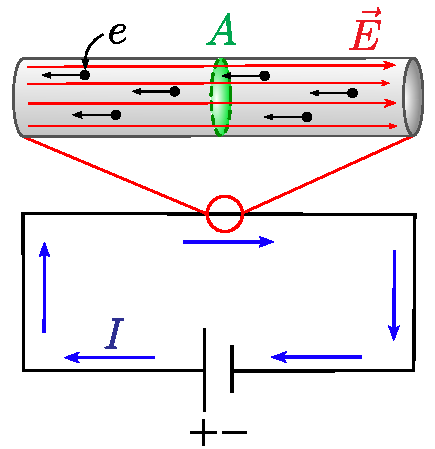
\includegraphics[scale = 0.9]{Figuras/Corriente-Electrica.pdf}
    \caption{Corriente eléctrica.}
    \label{fig:Corriente-Electrica}
\end{figure}

Entendemos por \textbf{corriente eléctrica} al flujo de portadores de carga a través de una superficie real o imaginaria. Estas cargas pueden ser electrones en un metal o en un tubo de rayos catódicos, o iones de un electrolito.

Si a través de cualquier corte transversal de área $A$  pasa una carga $dQ$ en un tiempo $dt$. Se define la \textbf{intensidad de corriente} como
\begin{shaded}
$$I:= \frac{dQ}{dt}.$$
\end{shaded}

La unidad de medida en el S.I es el \textit{ampère} ($A$), donde 
$$1 \, A = 1 \, \frac{C}{s}.$$

\textbf{Observación:} La corriente eléctrica es un escalar pero tiene sentido positivo o negativo.

\textbf{Propiedades de la corriente:}

\begin{enumerate}
\item La corriente eléctrica es la misma en todas las secciones transversales de un conductor, aún cuando la sección transversal sea diferente a lo largo del conductor.

\item La dirección de la corriente es la dirección en que se moverían las cargas positivas llamada \textit{corriente convencional}. Pero ojo: las partículas que transportan carga a través del alambre son los electrones libres, la convención ha permanecido por razones históricas.
\end{enumerate}

\subsection{Densidad de corriente}

Consideremos una superficie sobre la cual inciden cargas con densidad de carga $\rho$ moviéndose con velocidad $\Vec{v}$, cruzando un elemento de superficie (orientado) $d\Vec{S} = \hat{n} \,dS$, ver figura \ref{fig:Densidad-Corriente}.

\begin{figure}[H]
    \centering
    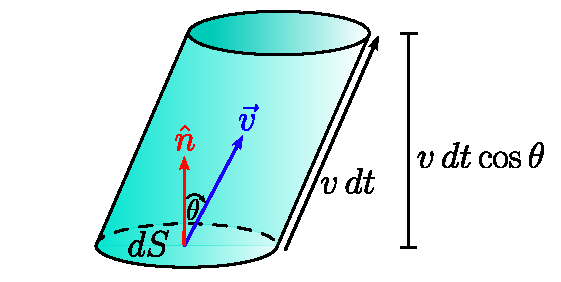
\includegraphics[scale = 0.95]{Figuras/Densidad-Corriente.pdf}
    \caption{Carga con densidad $\rho$ fluyendo con velocidad $\Vec{v}$ a través de un elemento de superficie $d\Vec{S}$.}
    \label{fig:Densidad-Corriente}
\end{figure}

La carga neta que atraviesa $dS$ en un intervalo $dt$ es
\begin{equation}
  dQ = \rho\,dV = \rho \underbrace{\,dS}_{\text{Base}} \underbrace{\,(v\,dt) \cos \theta}_{\text{Altura}}  = \rho (\Vec{v} \cdot \hat{n}) \,dS\,dt = \rho \Vec{v}\cdot d\Vec{S} \,dt. \label{Derivacion-J}  
\end{equation}

Se define la \textbf{densidad de corriente eléctrica} $\Vec{J}$ como
\begin{shaded}
   $$ \Vec{J}(\Vec{x},t) := \rho(\Vec{x},t) \Vec{v}(\Vec{x},t).$$
\end{shaded}

 La unidad de medida en el S.I. es $\left[\frac{A}{m^2} \right]$.

En otras palabras, la densidad de corriente es la
carga por unidad de tiempo y por unidad de superficie que atraviesa un elemento de área normal dado. Como consecuencia de la expresión \eqref{Derivacion-J}, la corriente eléctrica que atraviesa una superficie $S$ está dada por
\begin{shaded}
    $$I = \iint_S \Vec{J} \cdot d\Vec{S}.$$
\end{shaded}

\textbf{Observación:} Note que hemos escrito que los campos dependen de la posición y el tiempo, lo cual es cierto en general. Ahora bien, hasta el momento sólo consideraremos el estado estacionario, es decir, sin dependencia temporal.

\subsection{Corriente convencional}

En los comienzos de la Electrotecnia se creía que la corriente eléctrica en los metales consistía en el movimiento de las cargas positivas, en sentido contrario a los electrones. Afortunadamente la situación es equivalente ya que, como veremos, la densidad de corriente es igual para ambos tipos de portadores de carga.

Para iniciar nuestro estudio imaginemos un elemento de conductor en el que existen $n$ portadores de carga libres por unidad de volumen. Si el portador es positivo la carga es $e$ y si es negativo $-e$. En presencia de un campo eléctrico, los portadores de carga se moverán estacionariamente con una velocidad media o de arrastre, $\Vec{v}_a$ (portadores positivos) y $-\Vec{v}_a$ (portadores negativos), paralela y dependiente de él, ver figura \ref{fig:Corriente-Convencional}.

\begin{figure}[H]
    \centering
    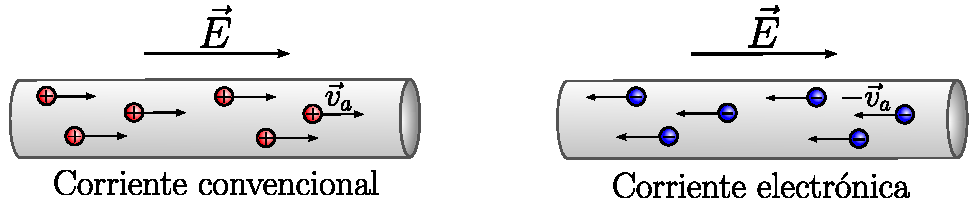
\includegraphics[scale = 0.89]{Figuras/Corriente-Convencional.pdf}
    \caption{Corriente convencional y electrónica.}
    \label{fig:Corriente-Convencional}
\end{figure}

Las densidades de corriente para el caso de la corriente convencional y la electrónica son, respectivamente,
$$\vec{J}_{+} = e\, n \,\vec{v}_{a}, \quad \Vec{J}_{-} = (-e) n (-\vec{v}_{a}) = e n \vec{v}_{a}.$$

Luego, las densidades de corriente son iguales.

\textbf{Observación:} Las carga convencionales no son los protones de los átomos de la red.

\section{Ecuación de continuidad}

La densidad de corriente $\vec{J}$ y la densidad volumétrica de carga $\rho$ son cantidades que están relacionadas por medio de una ecuación diferencial llamada \textbf{ecuación de continuidad}.

Consideremos un volumen $V$ arbitrario, encerrado por una superficie $\partial V$, en que la carga neta varía en el tiempo ($\rho = \rho(\vec{x},t)$). Entonces la corriente que entra en la superficie es
$$I = - \oiint_{\partial V} \vec{J} \cdot d\vec{S},$$

el signo menos es porque el diferencial de superficie $d\vec{S}$ siempre apunta hacia afuera en una superficie cerrada. Entonces, si $\vec{J}$ entra, $I = dQ/dt > 0$ lo que implica un aumento de cargas dentro del volumen. Pero, si $\vec{J}$ sale, $I = dQ/dt < 0$ lo que implica una disminución de cargas dentro del volumen.

Aplicando el teorema de Gauss,
\begin{equation}
I = - \oiint_{\partial V} \vec{J} \cdot d\vec{S} = - \iiint_V \vec{\nabla} \cdot \vec{J} \,dV. \label{Continuidad1}
\end{equation}

Como $I = dQ/dt$ y $Q = \iiint_V \rho \,dV$, se tiene que
\begin{equation}
I = \frac{d}{dt} \left( \iiint_V \rho(\vec{x},t) \,dV \right) \Rightarrow I = \iiint_V \frac{\partial \rho}{\partial t} \,dV.  \label{Continuidad2}
\end{equation}

Igualando \eqref{Continuidad1} y \eqref{Continuidad2}:
$$- \iiint_V \vec{\nabla} \cdot \vec{J} \,dV  = \iiint_V \frac{\partial \rho}{\partial t} \,dV \Rightarrow \iiint_V \left( \frac{\partial \rho}{\partial t} + \vec{\nabla} \cdot \vec{J} \right) \,dV = 0,$$

puesto que $V$ es arbitrario, entonces que la expresión anterior sea cero, implica que el integrando debe ser cero
\begin{shaded}
 $$\frac{\partial \rho}{\partial t} + \vec{\nabla} \cdot \vec{J} = 0.$$   
\end{shaded}

\textbf{Observación:} Para el caso de \textbf{corrientes estacionarias}, es decir, flujos de cargas continuos que han circulado desde siempre producto de un campo eléctrico estacionario, se tiene que
$$\frac{\partial \rho}{\partial t} = 0, \quad \frac{\partial \Vec{J}}{\partial t} = \Vec{0},$$

la ecuación de continuidad toma la forma
$$\vec{\nabla} \cdot \vec{J} = 0.$$

\begin{ejemplo}
Consideremos una densidad de corriente dirigida radialmente hacia afuera y que decrece exponencialmente con el tiempo, $\Vec{J} = \frac{1}{r} e^{-t} \,\hat{r}$. Calcular la densidad de carga.

\textbf{Solución:} Por la ecuación de continuidad,
$$- \frac{\partial \rho}{\partial t} = \vec{\nabla} \cdot \Vec{J} = \vec{\nabla} \cdot \left( \frac{1}{r} e^{-t} \,\hat{r}\right).$$

Usando la divergencia en coordenadas esféricas:
$$\Vec{\nabla} \cdot \Vec{J} = \frac{1}{r^2} \frac{\partial}{\partial r}  \left( r^2 \cdot\frac{1}{r} e^{-t} \right) = \frac{1}{r^2} e^{-t}.$$

Luego,
$$\frac{\partial \rho}{\partial t} = - \frac{1}{r^2} e^{-t}.$$

Integramos con respecto a $t$, recordando que, en general, la densidad depende de las coordenadas y el tiempo, aparecerá una constante de integración que depende de las coordenadas.
$$\rho(r,t) = \int - \frac{1}{r^2} e^{-t} \,dt + C(r) = \frac{1}{r^2} e^{-t} + C(r).$$

Si asumimos que la densidad se anula en un tiempo largo ($\rho \to 0$ cuando $t \to \infty$), encontramos que $C(r) = 0$. Por lo tanto,
$$\rho(r,t) = \frac{1}{r^2} e^{-t}.$$
\end{ejemplo}

\section{Ley de Ohm}

\subsection{Ley de Ohm microscópica}

Mucho antes de que se supiera de la existencia de átomos y electrones, Ohm estableció la ley experimental que lleva su nombre, y que hoy se escribe
\begin{shaded}
\begin{equation}
      \Vec{J}(\Vec{x}) = \sigma \Vec{E}(\Vec{x}), \label{Ohm-Micro}  
\end{equation}
\end{shaded}

donde $\sigma$ es la \textbf{conductividad} del medio (no confundir con la densidad de carga superficial). Su recíproco,
$$\rho = \frac{1}{\sigma}$$

es la \textbf{resistividad} (de nuevo, no confundir con la densidad de carga). \footnote{En algunos libros denotan la conductividad por $g$ y la resistividad por $\mu$.}

\textbf{Nota:} Esta forma de la ley de Ohm se conoce como \textit{ley de Ohm microscópica} y es una muy buena aproximación para una gran cantidad de materiales conductores.

La unidad de medida de la resistividad, en el S.I, es
\begin{equation*}
1 \left[ \frac{V}{A}\,m \right] = 1 [\Omega \,m]
\end{equation*}

donde $1 \, [\Omega] = 1 \, [V/A]$ es el \textit{Ohm}. 

A continuación entregaremos una visión microscópica a la ley enunciada con una interpretación de la conductividad.

Usando la segunda ley de Newton a un portador de carga $q$ de cualquier signo:
$$\vec{F} = m\vec{a} ~\Rightarrow~ q\vec{E} = m \frac{d\vec{v}}{dt},$$

la cual es válida hasta que el portador choca y se detiene. Este reinicia su trayectoria y vuelve a chocar y así sucesivamente (entre colisiones).

Definimos el \textbf{tiempo entre colisiones} $\tau$ tal que 
$$q\vec{E} = m \frac{\vec{v}_a}{\tau},$$

donde $\vec{v}_a$ es la velocidad de arrastre del portador.

Despejando la velocidad de arrastre,
$$\vec{v}_a = \frac{q \tau}{m} \vec{E}.$$

Definimos como \textbf{movilidad del portador} al factor $\mu := \frac{q \tau}{m}$, para así obtener
$$\vec{v}_a = \mu \vec{E}.$$

Entonces, la densidad de corriente se puede expresar como
$$\vec{J} = n q \mu \vec{E},$$

donde $n$ es la densidad de los portadores de carga por unidad de volumen. Comparando con \eqref{Ohm-Micro}, hemos encontrado una expresión microscópica para la conductividad:
$$\sigma = nq \mu  = \frac{n q^2 \tau}{m}.$$

Por lo tanto, la conductividad tiene que ver con la densidad de cargas de conducción $n$ y con el tiempo entre colisiones $\tau$.

\subsection{Ley de Ohm macroscópica}

Para que exista una corriente eléctrica debe existir electrones libres y una diferencia de potencial
$$V_{ab} = V_a - V_b = - \int_b^a \vec{E} \cdot d\vec{x} = \int_a^b \vec{E} \cdot d\vec{x}.$$

Para un metal, $\vec{E} = \rho \vec{J}$,  entonces
$$V_{ab} = \int_a^b \rho \vec{J} \cdot d\vec{x},$$

en que la densidad de corriente se obtiene de
$$I = \iint_S \vec{J} \cdot d\vec{S}.$$

Combinando estas dos ecuaciones se obtiene la ley de Ohm para los casos de interés. Por ejemplo, consideremos un cable de resistividad $\rho$, sección transversal $A$ constantes y largo $L$, ver figura \ref{fig:Ley-Ohm}. 

\begin{figure}[H]
    \centering
    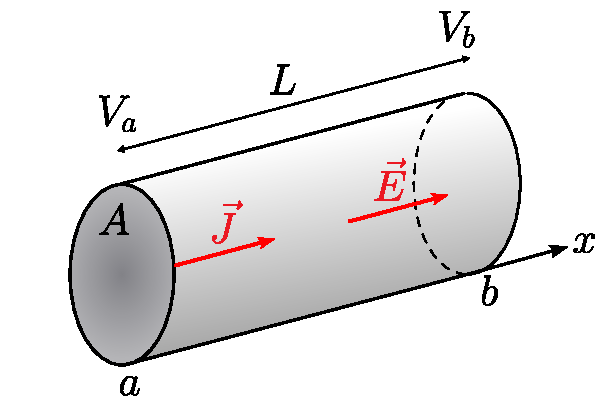
\includegraphics[scale = 0.7]{Figuras/Ley-Ohm.pdf}
    \caption{Alambre homogéneo que obedece la ley de Ohm.}
    \label{fig:Ley-Ohm}
\end{figure}

Además, asumiremos que $\Vec{E}$ y $\Vec{J}$ son uniformes, bajo estas condiciones, $\Vec{E}$ y $\Vec{J}$ son perpendiculares a la sección de área $A$ del cilindro. Así,
    \begin{align*}
        V_{ab} &= \int_a^b \rho \vec{J} \cdot d\vec{x} = \rho \int_0^L (J \,\hat{\imath})\cdot (dx \,\hat{\imath}) = \rho J L, \\
        I&= \iint_S \vec{J} \cdot d\vec{S} = \iint_S (J\,\hat{\imath}) \cdot (dS \,\hat{\imath}) = J \iint_S \,dS = JA.
    \end{align*}

Entonces,
$$V_{ab} = \rho JL = \rho \frac{L}{A} I.$$

Definimos la \textbf{resistencia eléctrica} por
\begin{shaded}
    $$R := \rho \frac{L}{A}.$$
\end{shaded}

Así, obtenemos la conocida \textbf{ley de Ohm macroscópica}
\begin{shaded}
    $$V_{ab} = RI.$$
\end{shaded}

La unidad de medida de la resistencia es el \textit{Ohm} ($[\Omega]$).

\textbf{Observaciones:}

\begin{enumerate}
\item  Estas expresiones son válidas solo para conductores homogéneos e isótropos de sección transversal uniforme sometido a un campo eléctrico uniforme. Si los campos no son uniformes, la resistencia puede ser definida de todas manera como $V/I$, donde $V$ es la diferencia de potencial entre dos superficies a distinto potencial del material, e $I$ es la corriente total que va del conductor positivo al negativo. Recordando que
$$V = - \int_{C} \Vec{E} \cdot d\Vec{x} ~~\text{y}~~ I = \oiint_S \Vec{J} \cdot d\Vec{S},$$

obtenemos que la resistencia está dada por
$$R = \frac{V}{I} = \frac{- \int_{C} \Vec{E} \cdot d\Vec{x}}{\oiint_S \Vec{J} \cdot d\Vec{S}} = \frac{- \int_{C} \Vec{E} \cdot d\Vec{x}}{\oiint_S \sigma \Vec{E} \cdot  d\Vec{S}}.$$

\item Cualquier material que al aplicarle una diferencia de potencial, satisface la relación $V = IR$, diremos que es \textit{óhmico}.

\item Para calcular la resistencia de una sección cónica, podemos usar la ecuación para una sección transversal uniforme considerando diferenciales de longitud :
$$dR = \rho \frac{dL}{A(L)}.$$
\end{enumerate}

\section{Combinaciones de resistencias}

Deseamos tener la resistencia total equivalente de dos combinaciones:

\begin{itemize}
\item[i)] \textbf{En serie:} En este caso la corriente $I$ que pasa por ambas resistencias es la misma.

\begin{figure}[H]
    \centering
    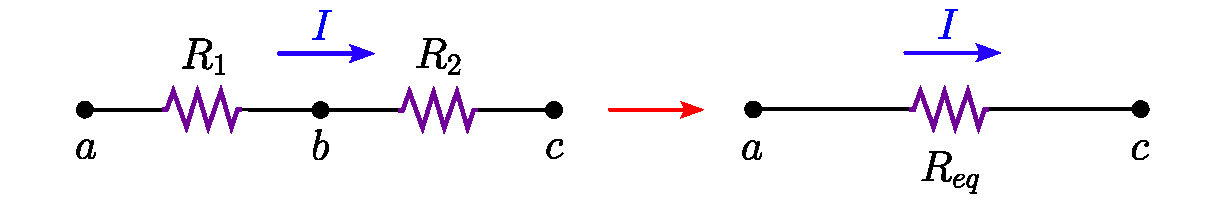
\includegraphics[scale = 0.7]{Figuras/Resistencias-Serie.pdf}
    \caption{Resistencias en serie}
    \label{fig:R-Serie}
\end{figure}

Dado que $V_{ac} = V_{ab} + V_{bc}$, ver figura \ref{fig:R-Serie}, por la ley de Ohm, tenemos que
\begin{align*}
  V_{ac} = V_{ab} + V_{bc} &\Rightarrow R_{eq} I = R_1 I + R_2 I \\
&\Rightarrow   R_{eq} = R_1 + R_2.  
\end{align*}


En general, para $n$ resistencias en serie,
\begin{shaded}
 $$R_{eq} = \sum_{i=1}^n R_i. $$  
\end{shaded}

\item[ii)] \textbf{En paralelo:}  En este caso ambas resistencias están a la misma diferencia de potencial, es decir, $V_{ab} = V_1 = V_2$, ver figura \ref{fig:R-Paralelo}. 

\begin{figure}[H]
    \centering
    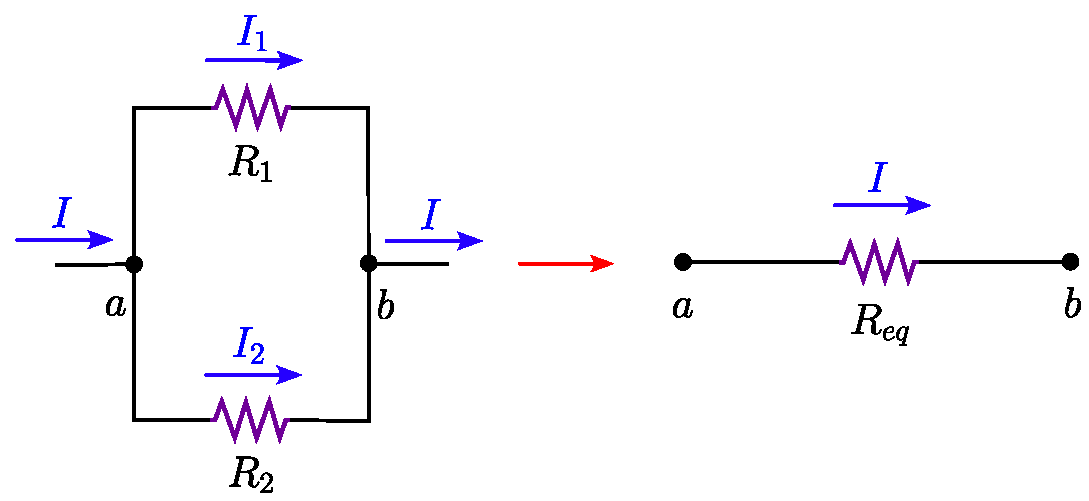
\includegraphics[scale = 0.7]{Figuras/Resistencias-Paralelo.pdf}
    \caption{Resistencias en paralelo.}
    \label{fig:R-Paralelo}
\end{figure}

Las corrientes se suman:
$$I = I_1 + I_2.$$

Por la ley de Ohm, sabemos que $I = \frac{V}{R}$. Luego,
\begin{align*}
   I = I_1 + I_2 
&\Rightarrow  \frac{V_{ab}}{R_{eq}} = \frac{V_{ab}}{R_1} + \frac{V_{ab}}{R_2} \\
&\Rightarrow \frac{1}{R_{eq}} = \frac{1}{R_1} + \frac{1}{R_2}. 
\end{align*}

En general, para $n$ resistencias en paralelo,
\begin{shaded}
    $$\frac{1}{R_{eq}} = \sum_{i=1}^n \frac{1}{R_i}.$$
\end{shaded}
\end{itemize}

\textbf{Observación:} Compare estos resultados con los obtenidos para capacitores en serie y en paralelo.

\section{Cálculo de resistencias*}

\begin{ejemplo}
    Un material de resistividad uniforme $\rho$ tiene forma de cuña tal como se muestra en la figura \ref{fig:Ej-1-Calculo-R}-(a). Encontrar la resistencia entre la cara $A$ y $B$.

    \begin{figure}[H]
        \centering
        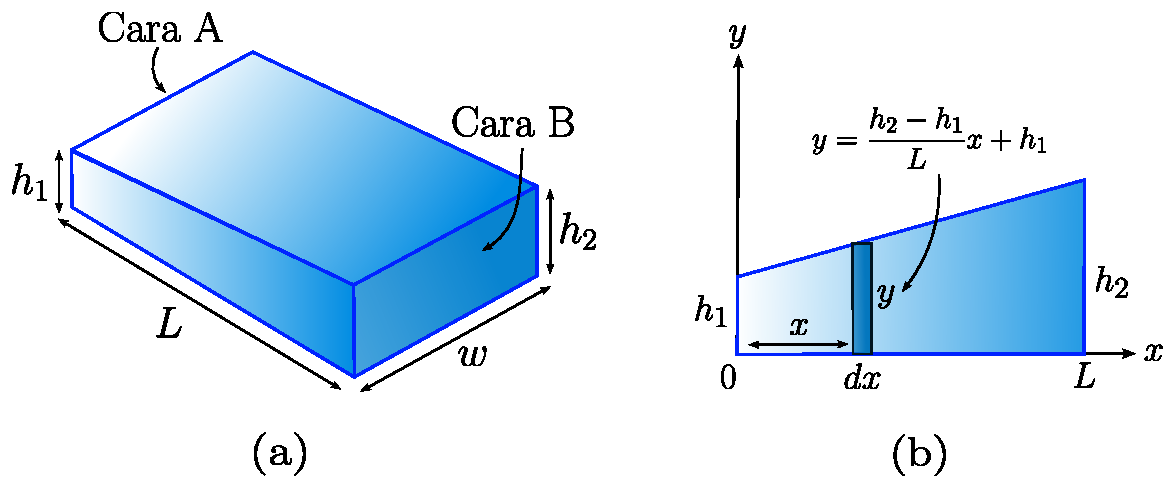
\includegraphics[scale = 0.7]{Figuras/Ej-1-Calculo-Resistencia.pdf}
        \caption{Resistencia de una cuña.}
        \label{fig:Ej-1-Calculo-R}
    \end{figure}

    \textbf{Solución:} Dado que el área transversal no es constante, no podemos utilizar directamente la ecuación $R = \frac{\rho L}{A}$. Entonces, procedemos a usar diferenciales considerando pequeños bloques de largo $dx$, altura $y$ y ancho $w$, ver figura \ref{fig:Ej-1-Calculo-R}-(b), de tal forma que el área transversal de cada elemento infinitesimal sea constante. 

    El área transversal de cada bloque es $A = wy$ y la resistencia es
    $$dR = \rho \frac{dx}{A} = \rho \frac{dx}{wy},$$

    donde $x$ e $y$ son variables a lo largo de la cuña. Para poder integrar esta expresión es necesario expresar $y$ como función de $x$. Utilizando el sistema coordenado de la figura \ref{fig:Ej-1-Calculo-R}-(b), la recta que pasa por los puntos $(0,h_1)$ y $(L,h_2)$ está dada por
    $$y = \frac{h_2 - h_1}{L}x + h_1.$$

    Así, 
    $$dR = \frac{\rho \,dx}{w \left( \frac{h_2 - h_1}{L}x + h_1\right)}.$$

    Cada uno de los bloques está en serie para formar la cuña, pues están a distinto potencial pero la intensidad de corriente que pasa a través de la cuña desde la cara $A$ a la $B$ es la misma. Entonces, integramos para calcular la resistencia total:
    $$R = \frac{\rho}{w} \int_0^L \frac{1}{\left( \frac{h_2 - h_1}{L}x + h_1\right)}  \,dx =  \left.  \frac{\rho}{w} \frac{1}{\frac{h_2-h_1}{L}} \ln \left(  \frac{h_2 - h_1}{L}x + h_1\right) \right|_0^L = \frac{\rho L}{w(h_2-h_1)} \ln \left(\frac{h_2}{h_1} \right).$$
\end{ejemplo}

\begin{ejemplo}
    Un semianillo de sección transversal rectangular de grosor $h$, con radio interior $a$ y exterior $b$, está hecho de un material conductor uniforme de resistividad $\rho$. Encuentre la resistencia eléctrica del semianillo entre sus caras rectangulares.

    \begin{figure}[H]
        \centering
        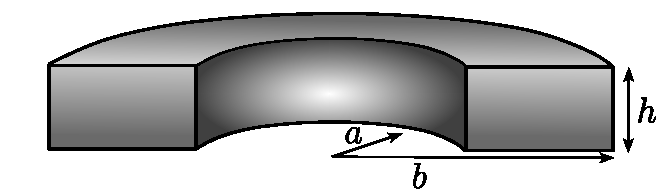
\includegraphics[scale = 0.75]{Figuras/Ej-2-Calculo-Resistencia.pdf}
        \caption{Resistencia de un semianillo.}
        \label{fig:Ej-2-Calculo-Resistencia}
    \end{figure}

    \textbf{Solución:} Dividimos en trozos infinitesimales el semianillo, para ello consideremos semianillos muy delgados de ancho $dx$ y altura $h$ tal como se muestra en la figura \ref{fig:Ej-2-Calculo-Resistencia}.

      \begin{figure}[H]
        \centering
        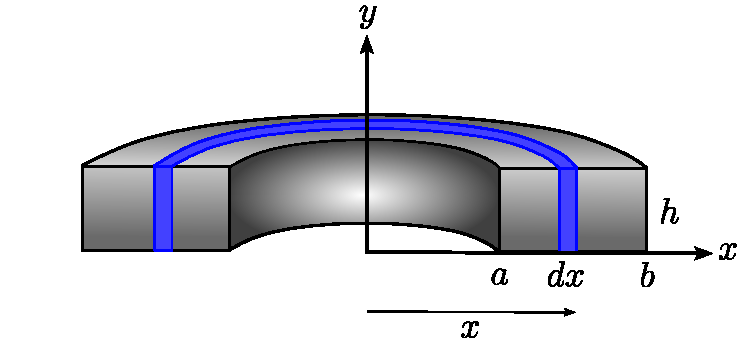
\includegraphics[scale = 0.75]{Figuras/Ej-2-Calculo-Resistencia-SistCoordenado.pdf}
        \caption{Resistencia de un semianillo.}
        \label{fig:Ej-2-Calculo-Resistencia-2}
    \end{figure}

    El área transversal de cada anillo es $A = h\,dx$ y la longitud que recorrerá la corriente es $L = \pi x$ (la mitad de una circunferencia). Así, su resistencia está dada por
    $$dR = \rho \frac{\pi x}{h\,dx}.$$

    Cada uno de los semianillos está en paralelo para formar el semianillo completo, pues están a igual potencial pero la intensidad de corriente no es la misma, pero si constante, en cada semianillo infinitesimal. Entonces, el recíproco de la resistencia total es
    $$\frac{1}{R} = \int_a^{b} \frac{h\,dx}{\pi \rho x} = \frac{h}{\pi \rho} \int_a^b \frac{1}{x}\,dx = \frac{h}{\pi\rho} \ln\left(\frac{b}{a}\right).$$

    Por lo tanto, la resistencia nos queda
    $$R = \frac{\pi \rho}{h \ln\left(\frac{b}{a} \right)}.$$
\end{ejemplo}

\section{Condiciones de borde*}
Sabemos que para corrientes estacionarias,
$$\Vec{\nabla} \cdot \Vec{J} = 0.$$

Por el teorema de Gauss, ésto implica que
$$\oiint_S \Vec{J} \cdot d\Vec{S} = 0.$$

Usando el mismo razonamiento hecho para el vector de desplazamiento eléctrico $\Vec{D}$ en la sección \ref{sec:Cond-Borde-Dielectricos}, donde teníamos que cuando no hay cargas libres $\oiint_S \Vec{D} \cdot d\Vec{S} = 0$ y se obtuvo la condición de borde $\Vec{D}_1 \cdot \hat{n} = \Vec{D}_2 \cdot \hat{n}$. En nuestro caso, la condición de borde para $\Vec{J}$ es
\begin{shaded}
    $$\Vec{J}_1 \cdot \hat{n} = \Vec{J}_2 \cdot \hat{n},$$
\end{shaded}

o bien,
\begin{shaded}
    $$ \sigma_1 \Vec{E}_1 \cdot \hat{n} =  \sigma_2 \Vec{E}_2 \cdot \hat{n}.$$
\end{shaded}

La condición de borde para el campo eléctrico es idéntica a la anterior:
$$\Vec{E}_1 \cdot \hat{t} = \Vec{E}_2 \cdot \hat{t},$$

pero como $\Vec{J} = \sigma \Vec{E}$, obtenemos una condición para las componentes tangenciales de $\Vec{J}$, a saber,
\begin{shaded}
    $$\frac{\Vec{J}_1 \cdot \hat{t}}{\sigma_1} = \frac{\Vec{J}_2 \cdot \hat{t}}{\sigma_2}.$$
\end{shaded}

\begin{ejemplo}
Considere un capacitador de placas cuadradas separadas a una distancia $d$. Dentro del capacitador existen dos medios con constantes dieléctricas y conductividades, $\varepsilon_1$, $g_1$ y $\varepsilon_2$, $g_2$. Los medios llenan la mitad del volumen del capacitador, ver figura \ref{fig:Ej-Cond-Borde-J}. Despreciando los efectos de borde determine los vectores $\Vec{J}$, $\Vec{E}$ y $\Vec{D}$ entre las placas conductoras en la condición de equilibrio.


    \textbf{Solución:} Despreciando los efectos de borde supondremos que los campos y densidades de corrientes tienen dirección en el eje $z$. Como estamos en la condición de equilibrio, no hay variación en la densidad superficial de carga entre los dos medios, por lo tanto se cumple la condición de un régimen permamente,
    $$\Vec{\nabla} \cdot \Vec{J} = 0,$$

    lo cual implica la continuidad de las componentes normales a la densidad de corriente:
    \begin{equation}
     \Vec{J}_1 \cdot \hat{n} = \Vec{J}_2 \cdot \hat{n}.   \label{Ej-CB-J-1}
    \end{equation}
    
    \begin{figure}[H]
        \centering
        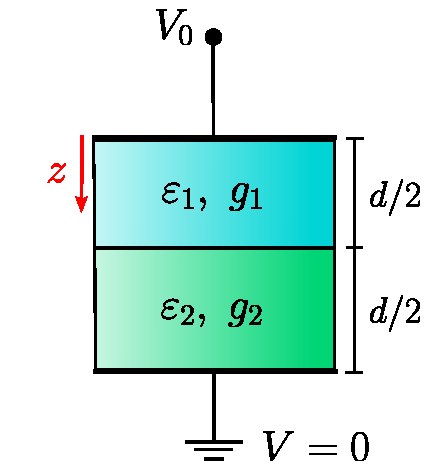
\includegraphics[scale = 0.7]{Figuras/El-Condicion-Borde-J.pdf}
        \caption{Capacitador compuesto.}
        \label{fig:Ej-Cond-Borde-J}
    \end{figure}
    
    Para los campos eléctricos, $\Vec{E}_1 = E_1 \,\hat{k}$ y $\Vec{E}_2 = E_2 \,\hat{k}$. De la ley de Ohm, se tiene que
    $$\Vec{J}_1 = g_1 \Vec{E}_1 ~~\text{y}~~ \Vec{J}_2 = g_2 \Vec{E}_2.$$

    Por lo tanto, de la ecuación \eqref{Ej-CB-J-1},
    \begin{equation}
        (g_1 E_1 \,\hat{z}) \cdot \hat{z} =  (g_2 E_2 \,\hat{z}) \cdot \hat{z} \Rightarrow g_1 E_1 = g_2E_2 \Rightarrow g_1 \vec{E}_1 = g_2 \Vec{E}_2. \label{Ej-CB-J-2}
    \end{equation}

    Por otro lado, sabemos que el potencial y  el campo eléctrico están relacionados por medio de la expresión
    $$V(B) - V_(A) = - \int_A^B \Vec{E} \cdot d\Vec{x}.$$

    En este caso, elegimos $A = (0,0,0)$, $B = (0,0,d)$ y $d\Vec{x} = dz\,\hat{k}$. Como $V(A) = V_0$ y $V(B) = 0$ (conectado a tierra), tenemos que
    $$V_0 = \int_0^{d/2} (E_1 \,\hat{k}) \cdot (dz \,\hat{k}) + \int_{d/2}^d (E_2 \,\hat{k}) \cdot (dz \,\hat{k}) =  \frac{d}{2} E_1 + \frac{d}{2} E_2.$$

   Luego,
   $$\Vec{E}_1 + \Vec{E}_2 = \frac{2V_0}{d} \,\hat{k}.$$

   Usando la condición \eqref{Ej-CB-J-2}, obtenemos que
   $$\vec{E}_1 = \frac{2g_2 V_0}{d(g_1 + g_2)} \,\hat{k} ~~\text{y}~~ \vec{E}_2 = \frac{2g_1 V_0}{d(g_1 + g_2)} \,\hat{k}.$$

   Luego, las densidades de corriente son
   $$\Vec{J}_1 = \Vec{J}_2 = \frac{2g_1 g_2 V_0}{d(g_1 + g_2)} \,\hat{k}.$$

   Para los vectores desplazamiento:
   \begin{align*}
       \Vec{D}_1 &= \varepsilon_1 \Vec{E}_1 = \frac{2 \varepsilon_1 g_2 V_0}{d(g_1 + g_2)} \,\hat{k} ,\\
       \Vec{D}_2 &= \varepsilon_2 \Vec{E}_2 = \frac{2 \varepsilon_2 g_1 V_0}{d(g_1 + g_2)} \,\hat{k}.
   \end{align*}
\end{ejemplo}

\section{Transferencia de energía en un circuito}

Supongamos que tenemos una fuente voltaica que entrega energía a un circuito compuesto de esta fuente y un dispositivo, ver figura \ref{fig:Energia-Circuito}.

\begin{figure}[H]
    \centering
    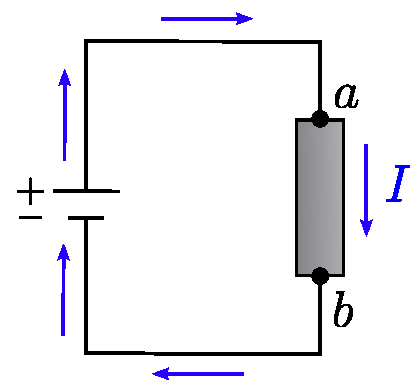
\includegraphics[scale = 0.8]{Figuras/Energia-Circuito.pdf}
    \caption{Transferencia de energía en un circuito.}
    \label{fig:Energia-Circuito}
\end{figure}

El terminal $a$ está conectado a un potencial mayor que el terminal $b$. Por lo tanto, una carga $dq$ que se mueve de $a$ hasta $b$ disminuye su energía potencial en
$$V_{ab} dq.$$

Como la energía siempre se conserva, la cantidad de energía que disminuye la carga $dq$ tiene que ser transformada en otra forma de energía en el artefacto.

En un tiempo $dt$ la energía transferida dentro del artefacto está dada por:
$$dU = V_{ab} dq = I V_{ab} dt.$$

Recordando la definición de \textbf{potencia}, se tiene que
\begin{shaded}
    $$P = \frac{dU}{dt} = I V_{ab},$$
\end{shaded}

la cual nos indica la rapidez con la que se entrega o se extrae energía hacia o desde un elemento de un circuito.

Si el dispositivo es óhmico:
\begin{shaded}
 $$P = IV_{ab} = I^2R = \frac{V_{ab}^2}{R}.$$   
\end{shaded}

La unidad de medida en el S.I. es el \textit{Watt}, donde
$$1 \, [W] = 1 \,[A V] = 1 \, [(C/s)(J/C)] = 1\, [J/s].$$

\section{Fuerza electromotriz}

En adelante vamos a analizar circuitos con corrientes estacionarias, es decir, corrientes en circuitos de \textbf{corriente continua}.

Para que un circuito se mantenga una corriente eléctrica, debe existir una fuente voltaica que proporcione la energía. Se llama \textbf{fuerza electromotriz} de la fuente a la energía por unidad de carga que ella entrega:
\begin{shaded}
    $$\varepsilon = \frac{dW}{dq},$$
\end{shaded}

con unidad de medida, en el S.I, $1 \, [V] = 1 \, [J/C]$.

\begin{figure}[H]
    \centering
    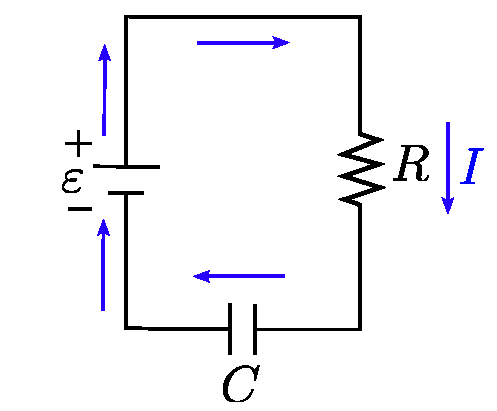
\includegraphics[scale = 0.75]{Figuras/fem.pdf}
    \caption{Fuerza electromotriz.}
    \label{fig:fem}
\end{figure}

De la figura \ref{fig:fem} vemos que el $+$ está a mayor potencial que el $-$ y los portadores positivos se mueven como muestran las flechas azules.

Aclaramos que el nombre fuerza es equivocado y se debe a razones históricas, no es una fuerza sino un voltaje. Habitualmente a la fuerza electromotriz se le llama \textit{fem}. 

De la definición de \textit{fem}, se tiene que
$$\varepsilon = \frac{dW}{dq} \Rightarrow dW = \varepsilon dq.$$

Dado que la potencia entregada por la fuente es $P = \frac{dW}{dt}$, entonces
$$\frac{dW}{dt} = \varepsilon \frac{dq}{dt} \Rightarrow \boxed{P = \varepsilon I}$$

Luego, $P$ es la potencia entregada por la fuente voltaica. Sabiamos que la potencia estaba definida por $P = IV$, entonces con ésto se demuestra que la \textit{fem} en realidad es una diferencia de potencial entre dos puntos.

\subsection*{Analogía gravitatoria}

En la figura \ref{fig:fem}, la fuente de fem realiza un trabajo sobre los portadores de carga. Esta energía almacenada en el trayecto como energía eléctrica, aparece luego como energía interna en la resistencia $R$. En la figura \ref{fig:Analogia-Gravitatoria}, una persona, por ejemplo, Darth Vader, al levantar las bolas de boliche desde el piso hasta la estantería (usando la `` fuerza ''), efectúa un trabajo sobre ellas. Esta energía se almacena en el trayecto como energía del campo gravitatorio. Las bolas ruedan lenta y uniformemente a lo largo de la estantería, cayendo por el extremo derecho dentro de un cilindro lleno de un medio viscoso. Se hunden hasta el fondo con una velocidad esencialmente constante (desde el mayor potencial $A$ al menor potencial $B$), para luego rodar de regreso a lo largo del suelo hacia la izquierda. La energía proporcionada por Darth Vader aparece al final como energía interna en el fluido viscoso, dando como resultado una elevación de la temperatura.

\begin{figure}[H]
    \centering
    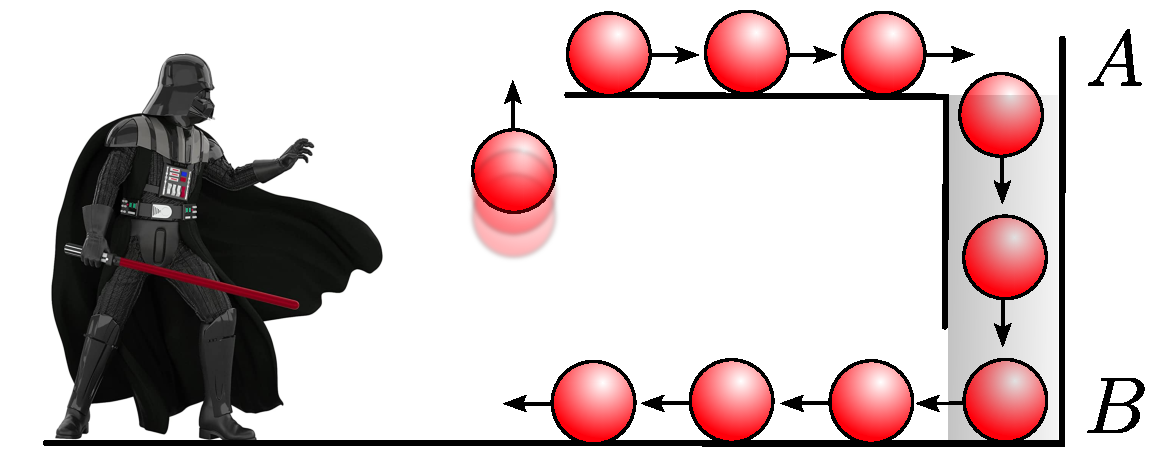
\includegraphics[scale = 0.59]{Figuras/Interpretacion-Fem.pdf}
    \caption{Analogía gravitatoria, en
la que el trabajo realizado por Darth Vader mantiene un flujo uniforme de bolas de boliche.}
    \label{fig:Analogia-Gravitatoria}
\end{figure}

\subsection*{Cálculo de la diferencia de potencial en un circuito cerrado}

\begin{itemize}
\item[a)] \textbf{Usando conservación de la energía:}

\begin{figure}[H]
    \centering
    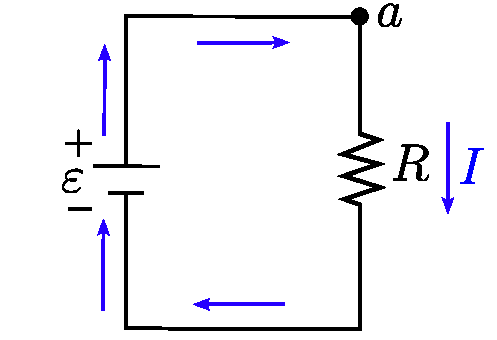
\includegraphics[scale = 0.75]{Figuras/Circuito-Cerrado.pdf}
    \label{fig:Circuito-Cerrado}
\end{figure}

La energía disipada en la resistencia en un tiempo $dt$ está dada por
$$I^2R \,dt.$$

Durante este mismo tiempo la fuente de \textit{fem} realiza un trabajo
$$dW = \varepsilon \,dq = \varepsilon I \,dt.$$

Usando el principio de la conservación de la energía:
$$\varepsilon I \,dt = I^2 R \,dt 
 \Rightarrow \boxed{\varepsilon - IR = 0}$$

Ésto nos dice que la suma algebraica de los cambios en el potencial encontrado en un recorrido completo del circuito cerrado es cero, lo cual se puede generalizar para cualquier circuito cerrado.

\item[b)] \textbf{Usando el concepto de potencial:}

Recorriendo el circuito en el sentido de la corriente, comenzando del punto $a$, con un potencial $V_a$, se tiene que
$$V_a - IR + \varepsilon = V_a \Rightarrow \boxed{\varepsilon -IR = 0}$$

La razón de porqué el potencial en la resistencia es negativo se debe a que en la resistencia ocurre una caída del potencial, es decir, las cargas al pasar por la resistencia, el potencial que tenían en $a$, disminuye en un valor de $IR$.

\end{itemize}

\section{Leyes de Kirchhoff}

Los cálculos hechos en la sección anterior se pueden sistematizar y generalizar en estas leyes para así resolver circuitos más complejos.

Antes de enunciar las leyes, veamos algunas definiciones previas:

\begin{itemize}
\item Llamamos \textbf{nodo} de un circuito al punto donde se unen 3 o más conductores.

\item Llamamos \textbf{rama} de un circuito a cualquier trayectoria  que une 2 nodos.

\item Llamamos \textbf{malla} de un circuito a un recorrido cerrado en él.
\end{itemize}

Con lo anterior, enunciemos las leyes:

\begin{enumerate}
\item \textbf{Ley de los nodos:} La suma algebraica de las corrientes que entran en un nodo es igual a las que salen.
\begin{shaded}
 $$\sum I_{entrante} = \sum I_{saliente}.$$   
\end{shaded}

\item \textbf{Ley de las mallas:} La suma algebraica de las diferencias de potencial en cualquier malla es cero.
\begin{shaded}
    $$\sum_n \varepsilon_n + \sum_k V_k = 0.$$
\end{shaded}

\end{enumerate}

Para la ley de las mallas debemos tener en cuenta lo siguiente:

\begin{itemize}
\item[i)] Si una resistencia se recorre en la dirección de la corriente, el cambio en el potencial es $-IR$ y si lo recorre en la dirección opuesta es $+IR$.

\item[ii)] Si una fuente de \textit{fem} se recorre desde el terminal negativo al positivo, el cambio en el potencial es $+\varepsilon$ y si se recorre en la dirección opuesta es $- \varepsilon$.
\end{itemize}

La figura \ref{fig:Recorrido-Circuito} resume lo expuesto.

\textbf{Observación:} La primera ley es consecuencia de la conservación de la carga y la segunda, de la conservación de la energía.

\begin{figure}[H]
    \centering
    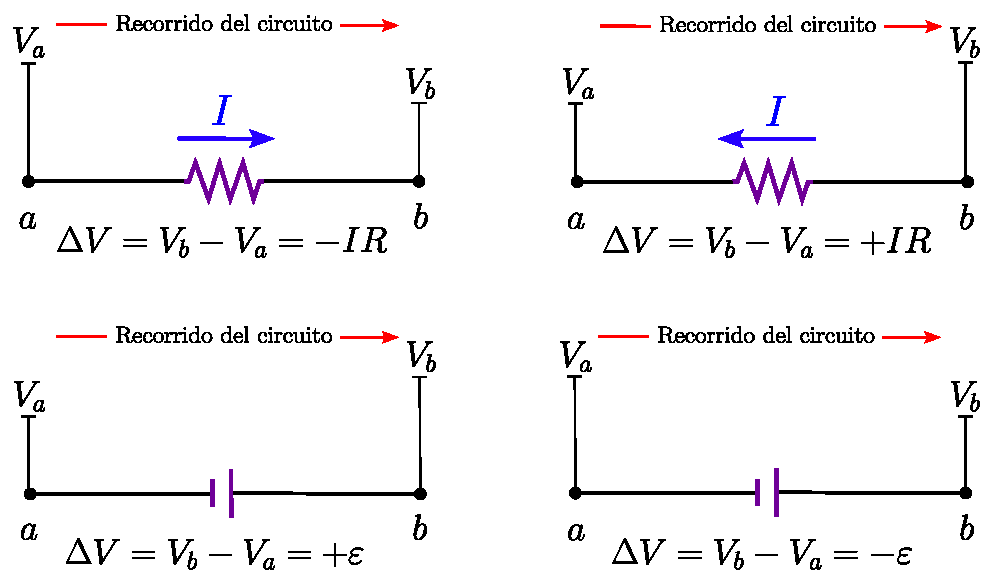
\includegraphics[scale = 0.8]{Figuras/Recorrido-del-circuito.pdf}
    \caption{Reglas para determinar las diferencias de potencial a través de una resistencia y una fem.}
    \label{fig:Recorrido-Circuito}
\end{figure}


\begin{ejemplo}[Resistencia interna de una fuente de \textit{fem}]

Las fuentes voltaicas pueden tener resistencia interna, la cual denotaremos por $r$. Nuestro objetivo será calcular la diferencia de potencial en los bornes de la batería, es decir, entre $a$ y $b$ conocidos los valores de $r$, $R$ y $\varepsilon$.

\begin{figure}[H]
    \centering
    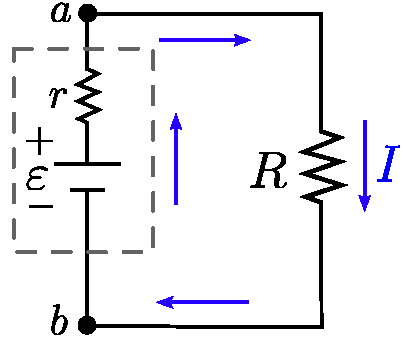
\includegraphics[scale = 0.8]{Figuras/Ej-1-Kirchoff.pdf}
    \caption{Resistencia interna de una fuente de fem.}
    \label{fig:resistencia-fem}
\end{figure}

Recorriendo este circuito en el sentido de la corriente desde el punto $b$ hasta el mismo punto $b$.
\begin{align*}
  V_b + \varepsilon - Ir - IR = V_b &\Rightarrow  \varepsilon - Ir - IR = 0 \\
&\Rightarrow I = \frac{\varepsilon}{r+R}.  
\end{align*}

Recorriendo este circuito en el sentido de la corriente, comenzando en $a$ hasta $b$.
\begin{align*}
  V_a - IR = V_b &\Rightarrow  V_a - V_b = IR \\
&\Rightarrow  V_{ab} = \frac{\varepsilon R}{r + R}.  
\end{align*}

\end{ejemplo}

\begin{ejemplo}
    Considere el circuito de la figura \ref{fig:Ej-2-Circuito},

\begin{figure}[H]
    \centering
    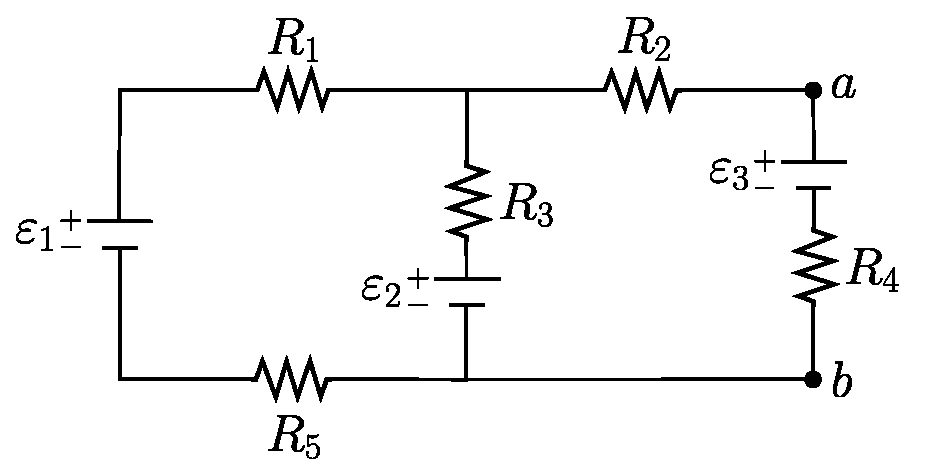
\includegraphics[scale = 0.67]{Figuras/Ej-2-Kirchoff.pdf}
    \caption{Circuito.}
    \label{fig:Ej-2-Circuito}
\end{figure}

donde $R_1 = 2 \,[\Omega]$, $R_2 = 4 \,[\Omega]$, $R_3 = 2 \,[\Omega]$, $R_4 = 2 \, [\Omega]$, $R_5 = 2 \,[\Omega]$, $\varepsilon_1 = 2 \,[V]$,$ \varepsilon_2 = 2 \,[V]$ y $\varepsilon_3 = 4 \,[V]$.

Determinar:
\begin{itemize}
\item[a)] La corriente en cada una de las resistencias.

\textbf{Solución:} Primero, reconocemos que tenemos dos mallas, $M_1$ y $M_2$, las cuales daremos sentidos, ver figura \ref{fig:Ej-2-Recorridos}. En segundo lugar, reconocemos que el circuito tiene dos nodos y tres ramas, y a cada rama asignamos un sentido de corriente, el cual es arbitrario.

\begin{figure}[H]
    \centering
    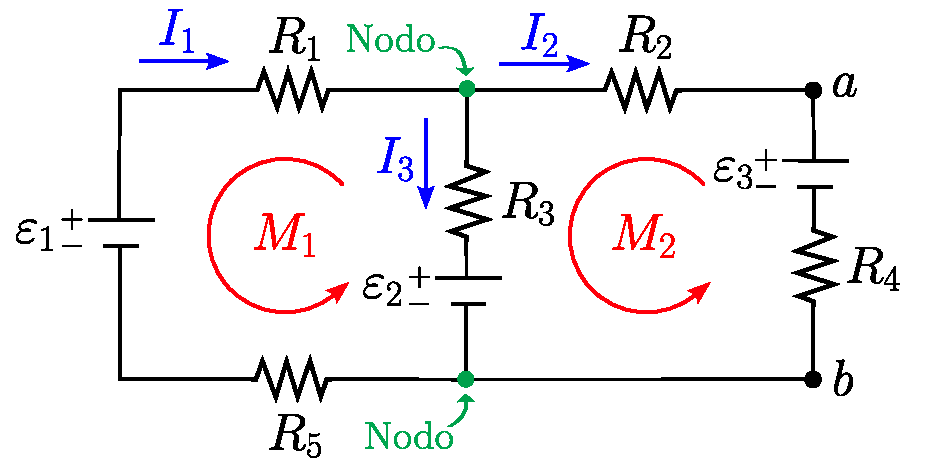
\includegraphics[scale = 0.67]{Figuras/Ej-2-Kirchoff-Recorridos.pdf}
    \caption{Recorridos de corriente y de malla.}
    \label{fig:Ej-2-Recorridos}
\end{figure}

Usando las leyes de Kirchhoff, tenemos la ecuación de nodos:
$$I_1 = I_2 + I_3$$

y las ecuaciones de mallas:
\begin{align*}
  - \varepsilon_1 + I_1 R_5 + \varepsilon_2 + I_3 R_3 + I_1 R_1 &= 0,\\
- I_3 R_3 - \varepsilon_2 + I_2 R_4 + \varepsilon_3 + I_2 R_2 &= 0 . 
\end{align*}

Reemplazando los datos en las 3 ecuaciones, se obtiene el siguiente sistema.
\begin{equation*}
\left\{ \begin{array}{ccl}
I_1 - I_2 - I_3 &=& 0  \\
-2 + 2I_1 + 2 + 2I_3 + 2I_1 &=& 0 \\
-2I_3 - 2 + 2I_2 + 4 +4I_2 &=& 0
\end{array} \right. \Leftrightarrow  \left\{ \begin{array}{ccl}
I_1 - I_2 - I_3 &=& 0  \\
2I_1 + I_3 &=& 0 \\
3I_2 - I_3 &=& -1
\end{array} \right.
\end{equation*}

Para resolver el sistema puede aplicar su método favorito. En nuestro caso aplicaremos el método de Eliminación de Gauss-Jordan aprendido en su lindo curso de Álgebra Lineal. La matriz ampliada del sistema es
\begin{equation*}
\left( \begin{array}{ccc|c}
1 & -1 & -1 & 0 \\
2 & 0 & 1 & 0 \\
0 & 3 & -1 & -1
\end{array} \right)  \longrightarrow \left( \begin{array}{ccc|c}
1 & -1 & -1 & 0 \\
0 & 1 & \frac{3}{2} & 0 \\
0 & 0 & 1 & \frac{2}{11}
\end{array} \right).
\end{equation*}

El sistema equivalente es
\begin{equation*}
\left\{ \begin{array}{ccl}
I_1 - I_2 - I_3 &=& 0  \\
I_2 + \frac{3}{2} I_3 &=& 0 \\
 I_3 &=&  \frac{2}{11}
\end{array} \right. ~\Leftrightarrow~ \left\{ \begin{array}{ccl}
I_1  &=& -\frac{1}{11} \\
I_2  &=& -\frac{3}{11} \\
 I_3 &=&  \frac{2}{11}
\end{array} \right. .
\end{equation*}

El signo negativo de las corrientes $I_1$ y $I_2$ nos dice que en realidad la corriente fluye en el sentido opuesto elegido.

\item[b)] La potencia disipada en la resistencia $R_3$.

\textbf{Solución:} La potencia disipada en $R_3$ está dada por:
$$P = I_3 V_3 = I_3^2 R_3 = \left( \frac{2}{11}\right)^2 \cdot 2 = \frac{8}{121} \,[W].$$

\item[c)] La diferencia de potencial entre los puntos $a$ y $b$.

\textbf{Solución:} Usando el concepto de la diferencia de potencial, hacemos un recorrido desde $a$ hasta $b$ pasando por la resistencia $R_4$.
\begin{align*}
  V_a - \varepsilon_3 - I_2 R_4 = V_b 
&\Rightarrow  V_a - V_b = \varepsilon_3 + I_2 R_4 \\
&\Rightarrow   V_a - V_b = 4 + \left( - \frac{3}{11} \right) \cdot 2  \\
 &\Rightarrow  V_{ab} =  \frac{38}{11} \,[V].  
\end{align*}

\end{itemize} 
\end{ejemplo}

\section{Instrumentos de medición}

A continuación se presenta un circuito compuesto por una \textit{fem} ($\varepsilon$) y dos resistencias ($R_1$ y $R_2$).

\begin{figure}[H]
    \centering
    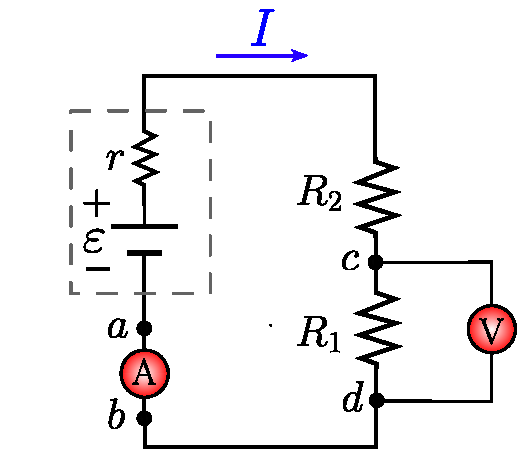
\includegraphics[scale = 0.8]{Figuras/Instrumentos-Medida.pdf}
    \caption{Instrumentos de medición.}
    \label{fig:Instrumentos}
\end{figure}

Nuestro objetivo es medir la corriente en los puntos $a$ y $b$ y el voltaje entre los puntos $c$ y $d$, para ellos son necesarios los siguientes instrumentos de medición:

\begin{enumerate}
\item El \textbf{amperímetro}, instrumento de medida de la intensidad de corriente, el cual debe ubicarse en serie con respecto al elemento al cual se le quiere medir la corriente. La resistencia interna de un amperímetro debe ser mucho menor a las resistencias que forman el circuito para así no alterar la corriente.

\item El \textbf{voltímetro}, instrumento de medida de diferencias de potencial, el cual debe ubicarse en paralelo al elemento al cual se le quiere determinar su voltaje. La resistencia del voltímetro debe ser mucho mayor que la resistencia a la cual se le desea medir la diferencia de potencial para que la corriente que pase por él sea ínfima.
\end{enumerate}

\section{Circuito RC}

En esta sección estudiaremos circuitos compuestos por una \textit{fem} ($\varepsilon$), una resistencia ($R$), un capacitador ($C$) y un interruptor ($S$), donde la carga y corriente no son constantes ($q = q(t)$ e $I = I(t)$).

Analizaremos dos etapas de acuerdo la posición del interruptor $S$, ver figura \ref{fig:Circuito-RC}.

\begin{itemize}
\item[i)] \textbf{Carga de un capacitador:}

Supongamos que el interruptor está en la posición 1.

\begin{figure}[H]
    \centering
    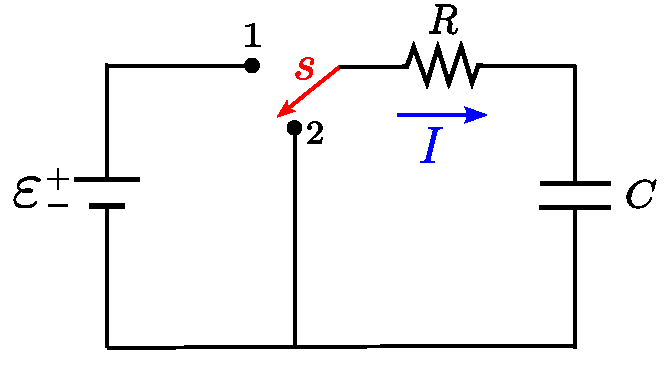
\includegraphics[scale = 0.75]{Figuras/Circuito-RC-Carga.pdf}
    \caption{Circuito RC.}
    \label{fig:Circuito-RC}
\end{figure}

Usando las leyes de Kirchhoff con un recorrido en el sentido de la corriente:
\begin{align}
  \varepsilon - IR - \frac{q}{C} = 0 
&\Rightarrow \varepsilon - R \frac{dq}{dt} - \frac{q}{C}  = 0 \nonumber \\
&\Rightarrow  R \frac{dq}{dt} + \frac{q}{C}  = \varepsilon \nonumber \\
&\Rightarrow  \frac{dq}{dt} +  \frac{q}{RC} =\frac{\varepsilon}{R}.   \label{eq:Circuit-RC}
\end{align}

Al resolver la ecuación diferencial ordinaria (EDO) lineal de primer orden, la solución general está dada por
$$q(t) = \varepsilon C + c_1 e^{-\frac{t}{RC}}, \quad c_1 \in \mathbb{R}.$$

Si $q(0) = 0$ (capacitador completamente descargado al inicio), entonces la constante $c_1 = - \varepsilon C$. Luego,
\begin{align*}
  q(t) &= \varepsilon C - \varepsilon C e^{-\frac{t}{RC}} = C \varepsilon (1 - e^{-\frac{t}{RC}}) \\
\Rightarrow ~ I(t) &= \frac{dq}{dt} = \frac{\varepsilon}{R}e^{-\frac{t}{RC}}.  
\end{align*}

Notemos que $\lim\limits_{t \to + \infty} q(t) =  C \varepsilon = Q$ es la carga máxima la cual se cargará el capacitador y para $t = 0$, $I(t) = \frac{\varepsilon}{R} = I_0$ es la corriente inicial y máxima la cual el sistema parte.

Definiendo la \textbf{constante capacitiva de tiempo} por $\tau_c := RC$.
\begin{shaded}
  $$q(t) = Q (1 - e^{-\frac{t}{\tau_c}}) ~~\mbox{y}~~ I(t) = I_0 e^{-\frac{t}{\tau_c}}.$$  
\end{shaded}

\textbf{Observación:} La constante capacitiva de tiempo es el tiempo en que ha aumentado la carga en el capacitador en un factor de $1 - e^{-1}$ ($\approx 63\%$) de su valor final $C\varepsilon$.

A continuación se presenta la gráfica general de $q$ e $I$ en el proceso de carga de un capacitador.

\begin{figure}[H]
    \centering
    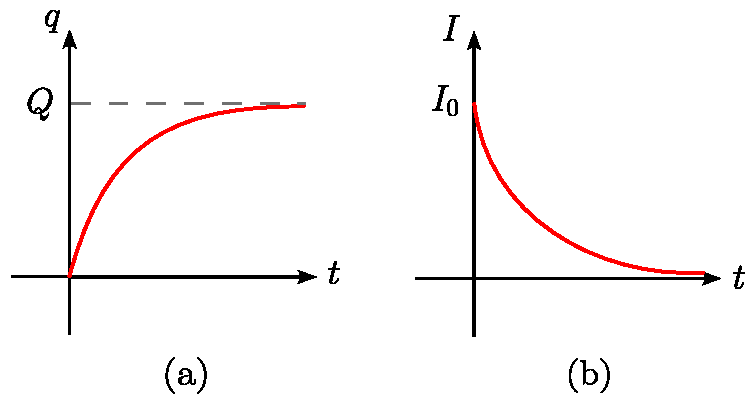
\includegraphics[scale = 0.9]{Figuras/Grafica-RC-Carga.pdf}
    \caption{Gráficas de carga en función del tiempo (a) y de la corriente en función del tiempo (b) para la carga de un capacitador en un circuito RC.}
    \label{fig:Grafica-RC-Carga}
\end{figure}

\item[ii)] \textbf{Descarga de un capacitador:}

Supongamos que el capacitador luego de cargarse, el interruptor es puesto en la posición $2$, ver figura \ref{fig:Circuito-RC}. En esta situación $\varepsilon = 0$ y el capacitador se descarga a través de la resistencia $R$.

La ecuación \eqref{eq:Circuit-RC} nos queda
$$\frac{dq}{dt} + \frac{q}{RC} = 0.$$

Al resolver la EDO lineal de primer orden, la solución general está dada por:
$$q(t) = c_1 e^{-\frac{t}{RC}}, \quad c_1 \in \mathbb{R}.$$

Si $q(0) = Q = \varepsilon C$ (inicialmente el capacitador), entonces la constante $c_1 = Q$.

Luego,
\begin{align*}
 q(t) &= Q e^{-\frac{t}{RC}}  \\
\Rightarrow ~ I(t) &= \frac{dq}{dt} = - \frac{Q}{RC}e^{-\frac{t}{RC}} = -  \frac{\varepsilon}{R}e^{-\frac{t}{RC}} = -I_0  e^{-\frac{t}{RC}}.   
\end{align*}

Reemplazando $\tau_c := RC$, encontramos que
\begin{shaded}
  $$q(t) = Q e^{-\frac{t}{\tau_c}} ~~\mbox{y}~~ I(t) = - I_0 e^{-\frac{t}{\tau_c}}.$$  
\end{shaded}

\textbf{Observación:} Para $t = \tau_c$, la carga del capacitador se reduce a $Qe^{-1}$, lo cual es de alrededor del $37\%$ de la carga inicial $Q$. 

El signo negativo de la corriente demuestra que la corriente fluye en dirección opuesta a la mostrada en la figura \ref{fig:Circuito-RC}. Esto es como debería ser, puesto que el capacitador se está descargando en lugar de cargarse.

A continuación se presenta la gráfica general de $q$ e $I$ en el proceso de carga de un capacitador.

\begin{figure}[H]
    \centering
    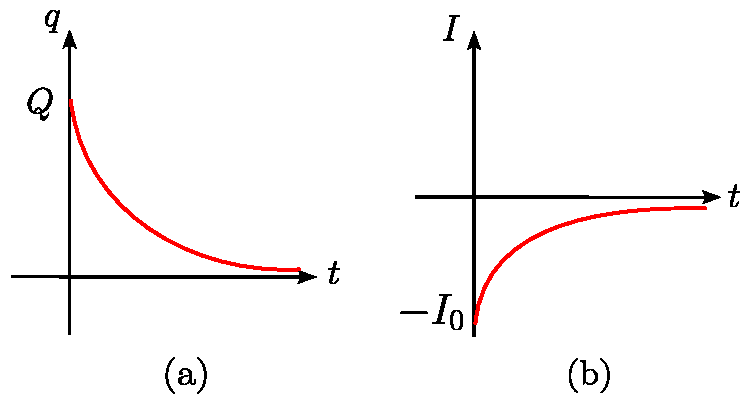
\includegraphics[scale = 0.9]{Figuras/Grafica-RC-Descarga.pdf}
    \caption{Gráficas de carga en función del tiempo (a) y de la corriente en función del tiempo (b) para la descarga de un capacitador en un circuito RC.}
    \label{fig:Grafica-RC-Descarga}
\end{figure}

\end{itemize}
